
\section{Introduction}
The purpose of this Completion Plan is to outline a detailed timeline for the remaining tasks required to finalise the Engineering Capstone Project, ensuring all milestones and deliverables are met within the reminder of the semester 2 2024. This plan revisits the project's deliverables and scope, taking into account recent changes and outlining strategies to overcome any logistical or technical barriers.

The original scope of the project aimed for the Aurora V rocket to reach an apogee of 10,000 feet as part of the Australian Universities Rocket Competition (AURC). However, due to unforeseen circumstances, the AURC has been canceled. This cancellation does not significantly impact our capstone project. The main changes include the use of a different rocket motor, resulting in a new expected apogee of 7,000 feet and an updated launch dates timeline which are detailed in the Gantt chart included in this plan.

Despite these adjustments, the project's core objectives and deliverables remain focused on the successful development and deployment of the rocket's avionics firmware, data collection, analysis tools and data verification. The detailed tasks and milestones have been adjusted accordingly to reflect these changes in scope and deliverables

\section{Completed Tasks}
The following is a summary of the milestones achieved in the project so far:

\begin{itemize}
    \item \textbf{Successful Launch of Aurora I}:
    \begin{itemize}
        \item \textbf{Avionics Data Logging}: The custom avionics system successfully logged flight data, including sensor readings from accelerometers, gyroscopes, and magnetometers.
        \item \textbf{Firmware Development}: Custom firmware and libraries were created for the Arduino Nano, facilitating clean data collection and storage.
        \item \textbf{Data Retrieval}: Data was successfully extracted from the onboard flash storage upon recovery of the rocket.
        \item \textbf{Preliminary Data Validation}: Initial comparison of sensor data with commercial flight computers (Blue Raven) indicated general agreement in acceleration, velocity, and attitude trends.
    \end{itemize}
    \item \textbf{Design and Implementation of Data frame Specification}:
\begin{itemize}
        \item \textbf{Structured Data Formats}: Developed structured formats for the collection and storage of sensor data, ensuring consistency when data logging to flash storage, and facilitating ease of post-flight data analysis for comparison against Blue Raven data.
\end{itemize}
    \item \textbf{Implementation and Verification of State Estimation Algorithms}:
    \begin{itemize}
        \item \textbf{Attitude Estimation}: Implemented attitude estimation using unit quaternion rotation, which provided accurate real-time orientation data of the rocket.
        \item \textbf{Velocity Estimation}: Developed a Kalman Filter model for velocity estimation, which enhanced the precision of velocity measurements by fusing data from multiple sensors.
    \end{itemize}
    \item \textbf{Aurora II Launch Outcomes}:
    \begin{itemize}
        \item \textbf{Barometric Data Collection}: Adjusted avionics A1 firmware to ensure correct collection and storage of barometric data, addressing issues identified during the Aurora I launch.
        \item \textbf{Telemetry Testing}: Conducted preliminary telemetry tests using ground communication hardware for real-time data transmission in future launches.
    \end{itemize}
    \item \textbf{Aurora III Firmware Structure}:
\begin{itemize}    
    \item \textbf{RTOS Task Planning}: Designed a high level RTOS architecture to efficiently manage time-critical tasks and handle the increased complexity of the system. This architecture ensures precise time management between different subsystems, allowing for the prioritisation of tasks and seamless integration of additional features as the firmware evolves. 
\end{itemize}
    \item \textbf{RTOS Implementation for Aurora III }:
    \begin{itemize}
        \item \textbf{High-Resolution Task}: Implemented a high-resolution task for capturing and processing sensor data at a frequency of 500Hz.
        \item \textbf{Low-Resolution Task}: Developed a low-resolution task for periodic data logging and communication.
        \item \textbf{State Update Task and Event Logging}: Created a state machine tasks for updating the rocket's state and logging significant flight events to trigger events based on the rockets state during flight.
        \item \textbf{Memory Flashing}: Implemented memory flashing routines to ensure data storage during flight similar to previous flights.
        \item \textbf{CAN Communications with Aerobrakes}: Established CAN communication protocols with the Aerobrakes subsystem, enabling coordinated control during flight.
    \end{itemize}
    \item \textbf{Kalman Filter Implementation}:
\textbf{State Estimation Enhancement}: Improved state estimation algorithms for accurate velocity and altitude measurements, integrating barometric and inertial sensor data through the Kalman Filter.

\end{itemize}

These completed tasks has formed the foundation for the project's next stages, ensuring that the avionics system is well-prepared for future launches and real-time data processing.


\section{Remaining Tasks}
This section details the remaining tasks required to complete the capstone project, with a focus on finalising all RTOS coding-related activities by Week 5 in preparation of upcoming Aurora launches. Due to the early launch dates and time constraints, most formal testing will be conducted post-flight. While these tests will occur after the launch, they are designed to provide valuable insights and guidance for future students undertaking similar projects, helping them understand the key considerations when testing firmware at the system level. Additionally, post-flight testing will address any edge cases and fill in code gaps to ensure a well-rounded code base.
\begin{figure}
    \centering
    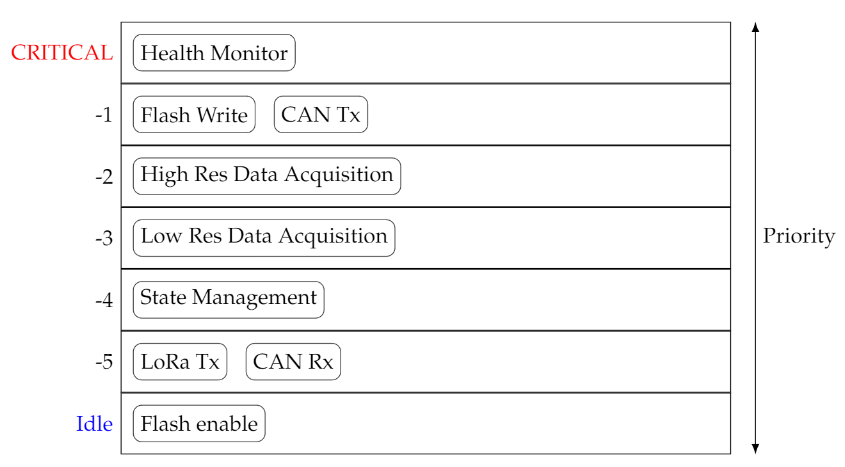
\includegraphics[width=1\linewidth]{img/RTOS-task-hierarchy.png}
    \caption{Avionics RTOS Task Hierarchy}
    \label{fig:enter-label}
\end{figure}

\subsection{Task 1: Finish Communications Tasks}
\textbf{Activity}: This task involves finalising the communication systems, specifically managing the LoRa and CAN protocols. The activities include adding and receiving messages from buffer queues to ensure data transmission and reception between the rocket's avionics system and ground stations or other subsystems. 

\textbf{Timeline}: Week 4-5

\textbf{Expected Completion Date}: 23rd August 2024

\textbf{Feedback Date}: 21st of August 2024

\subsection{Task 2: Implement UART Tasks}
\textbf{Activity}: Implement UART tasks to enable command and control functionalities. This includes developing UART command implementations for testing purposes and retrieving data from flash storage. Additionally, it involves manually setting states for debugging to ensure accurate system behaviour during various flight conditions. 

\textbf{Timeline}: Week 4-5

\textbf{Expected Completion Date}: 23rd August 2024

\textbf{Feedback Date}: 21st of August 2024

\subsection{Task 3: Verify Data from Flash}
\textbf{Activity}: Ensure that the message buffer does not interfere with the written data. This task involves verifying that the data readout from flash storage is valid and is not corrupted due to buffering issues or context switching from the RTOS. The aim is to confirm the integrity and sensibility of the stored data. 

\textbf{Timeline}: Week 4-5

\textbf{Expected}: 23rd August 2024

\textbf{Feedback Date}: 21st of August 2024

\subsection{Task 4: Implement GPS}
\textbf{Activity}: Implement the GPS task, utilising drivers already prepared by the Avionics, Ground Communications and Redundant Systems team. This task includes handling GPS data and ensuring it is correctly processed and sent to the LoRa communication system. Additionally, it involves setting up the GPS to operate in a non-blocking state, as it outputs a significant amount of data that is not required. 

\textbf{Timeline}: Week 4-5

\textbf{Expected Completion Date}: 23rd August 2024

\textbf{Feedback Date}: 21st of August 2024

\subsection{Task 5: Sensor Calibration}
\textbf{Activity}: Perform calibration of all sensors used in the rocket's avionics system. This ensures accurate readings and data integrity during flight. Calibration activities include setting up the sensors in a controlled environment recording any offsets that any of the sensors may output.

\textbf{Timeline}: Week 5

\textbf{Expected Completion Date}: 23rd August 2024

\textbf{Feedback Date}: 21st of August 2024

\subsection{Task 6: Implement Communications with Payload}
\textbf{Activity}: Develop, implement and test communication protocols between the avionics system and the payload subsystem. This ensures that critical data is shared and processed accurately between these systems during flight. 

\textbf{Timeline}: Week 5

\textbf{Expected Completion Date}: 23rd August 2024

\textbf{Feedback Date}: 21st of August 2024

\subsection{Task 7: Health Monitoring Task}
\textbf{Activity:} Develop a high-priority health monitoring task designed to ensure system health by actively monitoring the status of various avionics components. This task will wait for flags triggered by other tasks, such as sensor malfunctions or microcontroller failures. If a flag is set, the health monitoring task will immediately enter a RTOS critical section with top priority, executing predefined protocols to mitigate the issue. These protocols include switching to redundant sensors or microcontrollers to maintain system functionality. Additionally, the task will manage timeouts on polling to prevent unnecessary delays and will monitor conditions such as the flash buffer reaching capacity. 

\textbf{Timeline}: Week 5

\textbf{Expected Completion Date}: 23rd August 2024

\textbf{Feedback Date}: 21st of August 2024

\subsection{Task 8: Verify RTOS Task Execution}
\textbf{Activity}: Conduct thorough verification to ensure that all RTOS tasks are executing as scheduled. This involves monitoring the execution times and sequences of tasks to confirm that they adhere to the predefined schedule and priorities. 

\textbf{Timeline}: Week 5-7

\textbf{Expected Completion Date}: 13th of September 2024

\textbf{Feedback Date}: 18th of September 2024

\subsection{Task 9: Analyse Impact of Sample Loss}
\textbf{Activity}: Analyse the effect of senor data loss during errors and determine if the calculated state can recover from such loss. This involves creating scenarios where data samples are lost and observing the system's ability to maintain state estimation. 

\textbf{Timeline}: Week 5 - Mid Semester Break

\textbf{Expected Completion Date}: 6th of September 2024

\textbf{Feedback Date}: 11th of September 2024

\subsection{Task 10: Verify Kalman Gain as an Indicator}
\textbf{Activity}: Validate the use of Kalman gain as an indicator for system performance. This involves checking the accuracy of the Kalman gain values during different flight conditions and validating they provide meaningful insights. 

\textbf{Timeline}: Week 5 - Mid Semester Break

\textbf{Expected Completion Date}: 6th of September 2024

\textbf{Feedback Date}: 11th of September 2024

\subsection{Task 11: Design Error Determination for Redundancy}
\textbf{Activity}: Design logic for error determination to support redundancy. This involves creating algorithms that detect errors and switch to redundant sensors and microcontrollers to maintain functionality. 

\textbf{Timeline/Expected Completion}: Week 5 - Mid Semester Break

\textbf{Expected Completion Date}: 6th of September 2024

\textbf{Feedback Date}: 11th of September 2024

\subsection{Task 12: Dissimilar Sensor Configuration for Aurora V Hardware}
\textbf{Activity}: Configure and test dissimilar sensors to ensure they provide accurate data as per the primary suite of sensors. This involves configuring sensors with different specifications and integrating them into the system.

\textbf{Timeline}: Week 5

\textbf{Expected Completion Date}: 23rd August 2024

\textbf{Feedback Date}: 21st of August 2024

\subsection{Task 13: Testing and Validation of Sensors and System Testing}
\textbf{Activity}: This task involves conducting comprehensive testing and validation of all sensors ensuring that each component performs accurately under expected flight conditions. The testing procedures will include the use of laboratory equipment such as shake tables and a vacuum chamber for barometric sensors. By doing so, conditions can be simulated to verify RTOS tasks. 

\textbf{Sensor Functionality and Edge Case Testing}
\begin{itemize}
    \item \textbf{Accelerometer Testing}: The accelerometers will be subjected to high and low G-force tests using a shake table. This will verify that the sensor outputs are proportional to the applied vibrations across the expected operating range. 
    \item \textbf{Gyroscope Testing}: Gyroscopes will be tested using a driving simulator to validate their outputs are proportional to known rotation rates. A bias stability test will measure the drift over time, ensuring it remains within acceptable limits.
    \item \textbf{Barometer Testing}: Barometric sensors will undergo pressure validation in a vacuum chamber to simulate the pressure changes expected at an apogee of 7,000 feet. This includes verifying the accuracy of pressure readings against a Blue Raven flight computer. Additionally, temperature validation will be conducted in a temperature-controlled chamber to ensure the sensor compensates for temperature variations.
    \item \textbf{GPS Testing}: The GPS will undergo stationary and dynamic accuracy tests. The stationary test will verify the GPS maintains stable position data in a fixed location, while the dynamic test will ensure it accurately tracks movement, such as on a moving vehicle.
\end{itemize}

\textbf{Mission Simulation Testing}
\begin{itemize}
    \item \textbf{State Estimation Simulation Testing}: Simulated flight conditions will be used to validate state estimation algorithms, ensuring they accurately calculate position, velocity, and orientation during flight. This includes testing the apogee detection system to ensure it triggers recovery deployment at the correct altitude.
    \item \textbf{Aerobrakes Testing}: Aerobrakes will be tested under simulated flight conditions to verify their deployment. 
    \item \textbf{Recovery Deployment}: The recovery system will be tested to ensure they deploy correctly at apogee. Indicators like LEDs will be used as a test to confirm that the recovery is triggered at the correct time before recovery is connected to avionics. 
\end{itemize}

\textbf{Timeline}: Week 6-11

\textbf{Expected Completion Date}: 13th of October 2024 (all testing)

\textbf{Feedback Date}: 16th of October 2024

\subsection{Task 14: Redundancy Testing}
\textbf{Activity}: Conduct hardware-level testing to verify the redundancy mechanisms. This involves working closely with Avionics, Ground Communications and Redundant Systems team to design and implement tests that test the redundant systems function correctly in case of primary system failures. 

\textbf{Timeline}: Week 5-7

\textbf{Expected Completion Date}: 13th of September 2024

\textbf{Feedback Date}: 18th of September 2024

\subsection{Task 15: Documentation of Firmware}
\textbf{Activity}: Document all firmware developed for the project, including detailed descriptions of functionalities, configurations, and usage instructions through Doxgyen. This ensures that future teams or stakeholders can understand and utilise the firmware effectively. 

\textbf{Timeline}: Week 1-11

\textbf{Expected Completion Date}: 20th of October 2024 

\textbf{Feedback Date}: 16th of October 2024

\clearpage 
\begin{landscape}
\thispagestyle{empty} 
\begin{figure}[!htbp] 
    \centering
    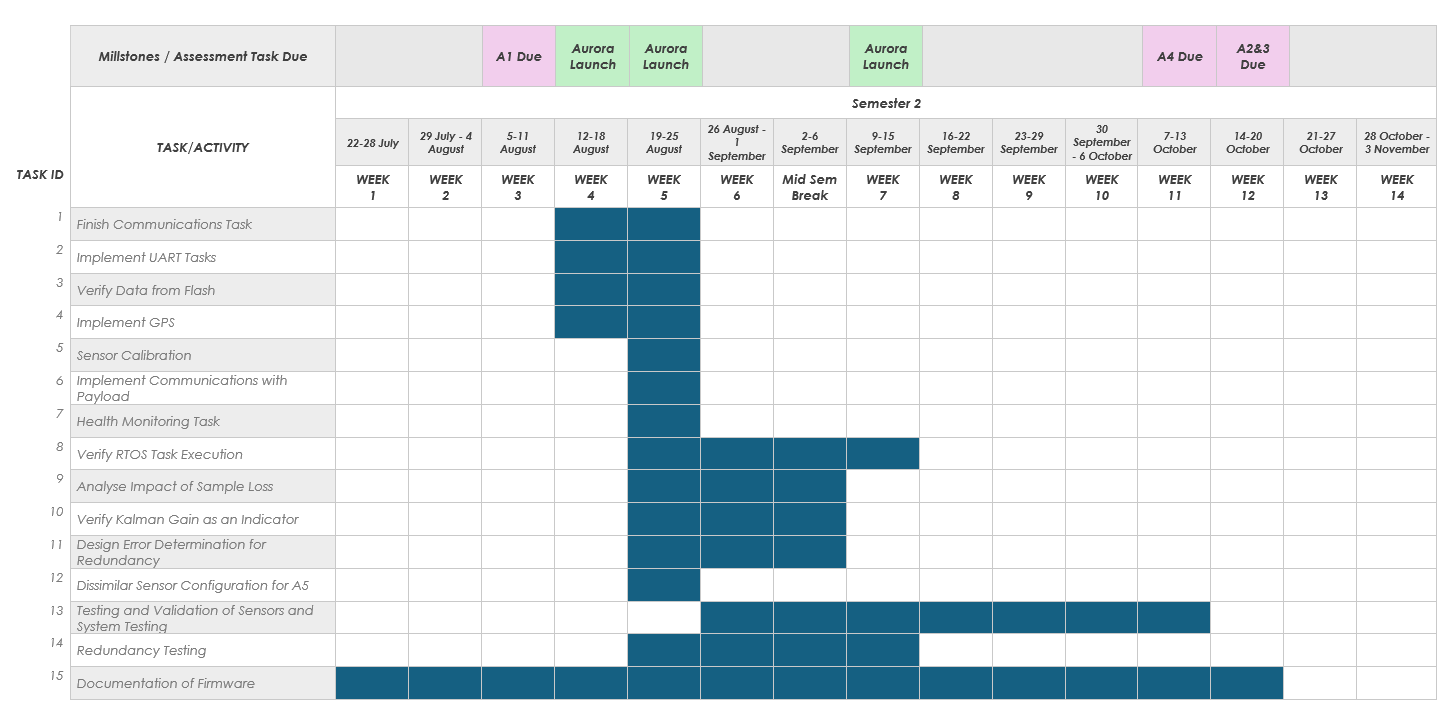
\includegraphics[width=\paperheight, height=\paperwidth, keepaspectratio]{img/Gantt-Chart-CP.png} 
    \caption{Gantt Chart - Project Timeline}
    \label{fig:Gantt Chart}
\end{figure}
\end{landscape}

\clearpage 



\section{Challenges}
Below are several challenges that have been identified that could potentially impact the timely and successful completion of the remaining tasks. This section outlines these challenges, and the strategies developed to overcome them.

\subsection{Time Management and Early Launch Dates}
The launch dates scheduled for this semester present a significant time management challenge as they are primarily within the first half of the semester. With limited time to complete all coding tasks and prepare for the launch, there is a risk of falling behind schedule or incomplete tasks. To address this, certain tasks will be prioritised which mainly focus on completing all RTOS coding-related tasks by Week 6 before the 24th of August launch. In addition to prioritisation, scheduling practices will be utilised, including the use of Gantt charts to map out the timeline for each task and weekly capstone meetings to monitor progress. 

\subsection{Communications and Collaboration with Avionics, Ground Communications, and Redundant Systems Teams}
Effective communication and collaboration with the Avionics, Ground Communications, and Redundant Systems teams is key for the successful integration aspect of the rocket. Design conflicts between the hardware and firmware may pose problems. To address this, the team has established regular coordination meetings to discuss progress, align on requirements, and address any dependencies. Clear and detailed documentation of all requirements, progress, and changes is maintained to keep everyone on the same page. 

\subsection{Lead Times for Accessing Laboratory Equipment}
Access to specialised laboratory equipment, such as shake tables and vacuum chambers, is critical for testing and validation. However, the process of securing this equipment involves navigating approval processes, including consultations with RMIT technical staff and completing detailed activity and equipment risk assessments. To address this, the team has initiated the approval process well in advance, working closely with technical staff to ensure all safety and procedural requirements are met. Furthermore, a flexible testing schedule has been developed to accommodate any delays in equipment availability. 

\subsection{Code Bugs and Unexpected RTOS Behaviour}
Potential code bugs and unexpected RTOS behaviour pose significant risks, especially close to launch dates. Early testing procedures of the RTOS code will be conducted to identify and resolve issues before they become critical. Regular consultations with project supervisor Dr. Glenn Matthews provide expert guidance on complex issues. Debugging protocols, including RTOS live debugging tools, systematic code reviews, and peer testing, are in place to address any problems, reducing the likelihood of significant delays.

\subsection{Availability of Avionics Hardware for Development}
Another significant challenge anticipated during the remainder of the project is the potential limited availability of the Avionics boards, which could impact the upcoming Aurora IV and Aurora V launches. During the Aurora III development of firmware, the team faced a similar issue, where they were reliant on the Avionics, Ground Communications, and Redundant Systems team to provide the necessary hardware. With only one Aurora III board available, the delay in receiving this avionics board reduced the time available for development and testing which ultimately resulted in unreliable features. This constrained testing period limited the ability to identify and resolve issues before the launch. To mitigate similar challenges for Aurora IV and Aurora V launches, the team will proactively coordinate with the relevant teams to ensure earlier access to the hardware. Additionally, the project timeline has been adjusted to prioritise critical tasks. These measures aim to minimise the impact of hardware availability constraints on the rocket's success. 

